\chapter{Feature Extraction}

As an acoustic wave propagated through space over time, the speech signal is not
appropriate to be evaluated by the speaker verification system. In order to deliver
decent outcomes, a good parametric representation must be provided to the system.
This task is performed by the feature extraction process, which transforms a speech
signal into a sequence of characterized measurements (features). As stated in
\autocite{davis.mermelstein.1980}, the usual objectives in selecting a representation
are (1) to compress the speech data by eliminating information not pertinent to
the phonetic analysis of the data, and (2) to enhance those aspects of the signal
that contribute significantly to the detection of phonetic differences. According
to \autocite{wolf.1972} the ideal features should:

\begin{itemize}\itemsep0pt\parskip0pt
    \item occur naturally and frequently in normal speech;
    \item be easily measurable;
    \item vary as much as possible among speakers, but be as consistent as possible
    for each speaker;
    \item not change over time or be affected by the speaker's health;
    \item not be affected by reasonable background noise nor depend on specific
    transmission characteristics;
    \item not be modifiable by conscious effort of the speaker, or, at least, be
    unlikely to be affected by attempts to disguise the voice.
\end{itemize}

Features may be categorized based on vocal tract or behavioral aspects, divided
in (1) short-time spectral, (2) spectro-temporal, (3) prosodic and (4) high
level \autocite{pinheiro.2013}. Short-time spectral features usually are calculated
using millisecond length windows and describe the voice spectral envelope, composed
of supralaryngeal properties of the vocal tract, e.g. timbre. Prosodic and
spectro-temporal occur over time, e.g. rhythm and intonation, and high level features
occur during the conversation, e.g. accents.

The parametric representations evaluated in \autocite{davis.mermelstein.1980} may
be divided into those based on the Fourier spectrum, Mel-Frequency Cepstrum
Coefficients (MFCC) and Linear Frequency Cepstrum Coefficients (LFCC), and those
based on the Linear Prediction Spectrum, Linear Prediction Coefficients (LPC),
Reflection Coefficients (RC) and Linear Prediction Cepstrum Coefficients (LPCC).
The better evaluated representation was the MFCC, with minimum and maximum accuracy
of 90.2\% and 99.4\% respectively, leading to its choice as the parametric
representation in this work.


\section{Mel Frequency Cepstral Coefficient}

MFCC is the most used parametric representation in the area of voice processing,
due to its similarity with the human ear operation. Despite the fact the ear is
divided in three sections, i.e. outer, middle and inner ears, only the last is
mimicked. The mechanical pressure waves produced by the hammer, the anvil and the
stirrup is received by the cochlea (\figureref{cochlea}), a spiral-shaped cavity
with a set of inner hair cells (basilar membrane) that converts motion to neural
activity throught a non-uniform spectral analysis \autocite{rabiner.schafer.2007}.
This activity is then passed to the pattern recognition existent in the brain.

\begin{figure}[ht]
    \centering
    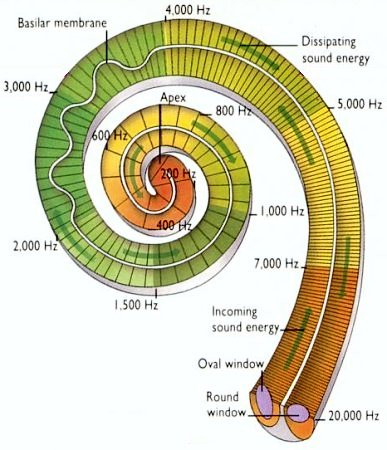
\includegraphics{cochlea}
    \caption{\captiontext{Cochlea divided by frequency regions.}}
    \label{fig:cochlea}
\end{figure}

A key factor in the perception of speech and other sounds is \emph{loudness}, a
quality related to the physical property of sound pressure level. Loudness is
quantified by relating the actual sound pressure level of a pure tone (in dB
relative to a standard reference level) to the perceived loudness of the same
tone (in a unit called phons) over the range of human hearing (20 Hz–20 kHz)
\autocite{rabiner.schafer.2007}. This relationship is shown in \figureref{loudness}.

\begin{figure}[ht]
    \centering
    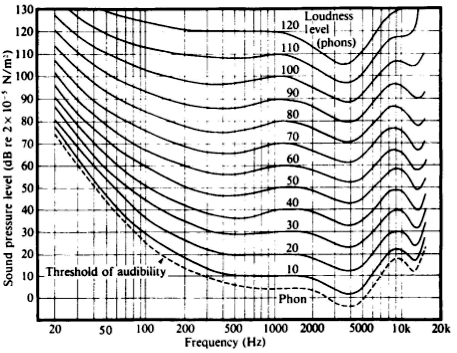
\includegraphics[scale=0.45]{loudness}
    \caption{\captiontext{Loudness level for human hearing.}}
    \label{fig:loudness}
\end{figure}


\subsection{The Mel Scale}


\subsection{Cepstrum}


\subsection{Extraction Process}


\subsubsection{Pre-emphasis}